The operation of filling bottles, from those of drinkable waters to containers of washing machine detergent, is highly automated. The high volume and low production cost requirements of these products make automation the only viable option. This report features a system capable of operating with different types of containers and varied liquid materials. The report also dives deep into a program that simulates the production line of bottled liquids. With some adaptations the program can be used to operate on the physical implementation of the system.

The system uses two feeders, one for bottles and one for liquids. When operating, the bottles are moved into a container and get rinsed, filled and caped. Finally the bottles of the same type and liquid, grouped together, are made available to packaging. To operate, the system uses a PLC program that verifies the count of bottles in the feeder to coordinate with moving of products to the conveyor and verifies volume of liquid available to coordinate with filling of bottles.

Other than the two feeders, the system requires a set of colored button devices, a bottle filling machine, a bottle conveyor and the PLC itself. The PLC used is Rockwell's model 5069-L306ER, with models 5069-IB6F and 5069-OB16 as input and output modules.

$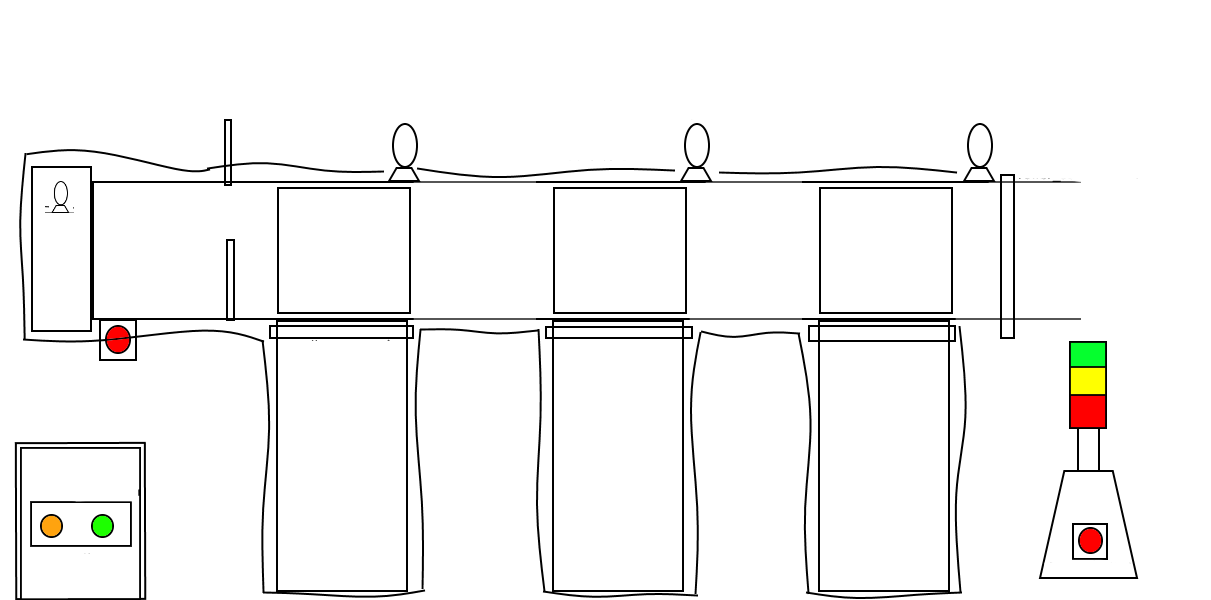
\includegraphics[scale=0.5]{../external/system_graphics_basic.png}